\documentclass[a1,portrait]{a0poster}

\usepackage[T1]{fontenc}
\usepackage[utf8]{inputenc}
\usepackage{url}
\usepackage{graphicx}
\usepackage{color}
\usepackage[francais]{babel}
\usepackage[left=2cm,right=2cm,bottom=2cm,top=0cm]{geometry}
\usepackage{flowfram}
\usepackage{template_poster}
\usepackage[bottom]{footmisc}

\AtBeginDocument{\def\labelitemi{$\bullet$}}
\AtBeginDocument{\def\labelitemii{$\circ$}}
\AtBeginDocument{\def\labelitemiii{--}}
%\AtBeginDocument{\def\labelitemiv{$\bullet$}}

\newcommand{\todo}[1]{\textbf{\textit{\color{red} #1}}}

\pdfinfo{
/Author (ASTUPS)
/Title (Conseils de Bricolage - v1.0)
/CreationDate (D:20141022)
/Creator (ASTUPS)
}

\title{Conseils de Bricolage}
\author{ASTUPS\\{\small Association des Sciences et Techniques de l'Université Paul Sabatier}}
\date{2014/2015 - v1.0}

%--------------------------------
% Edit flowfram options to create two columns, change the margin, ...
\setlength{\vcolumnsep}{\baselineskip}
\setlength{\columnsep}{\baselineskip}

\twocolumntop{static}{25cm}

\setstaticframe{1}{label={title}}


\begin{document}
\thispagestyle{empty}

\begin{staticcontents*}{title}
\maketitle

\newcommand{\tailleRegles}{\Large}
\section{Considérations Générales}
Lorem ipsum dolor sit amet, consectetur adipiscing elit. Nulla enim quam, porttitor sed massa vel, aliquet sagittis tortor. Suspendisse est eros, faucibus non vehicula eget, rutrum at purus. Aliquam auctor vehicula purus, consequat luctus lectus iaculis ultrices. Aliquam tempor dictum ullamcorper. Ut a facilisis lorem, vel tempus eros. Sed elit odio, feugiat vel molestie id, congue in nisl. Aliquam id erat non mi dapibus vulputate. Suspendisse potenti. Aenean tincidunt porta dapibus. Donec euismod eleifend urna, nec pharetra ex iaculis quis.


\end{staticcontents*}

\small

\def\tailleImageTournevis{0.3\columnwidth}
\def\formCoefficient{0.3}
\section*{Tournevis et Clés}
\begin{minipage}{0.8\columnwidth}
\textbf{Sens de vissage~:} Universellement, le sens horaire sert à visser, le sens inverse pour dévisser.
%\todo{\\footnote{\textbf{Faciliter le serrage ou desserrage~:} Il existe un dégrippant permettant de débloquer vis et écrous, il s'agit du WD-40.}}.

\end{minipage}
\hspace{0.06\columnwidth}
%\begin{minipage}[][][c]{0.2\columnwidth}
%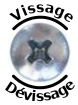
\includegraphics[width=\tailleImageTournevis]{pics/sens-vissage.pdf}
\begin{minipage}[][][c]{0.12\columnwidth}
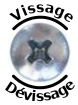
\includegraphics[width=\columnwidth]{pics/sens-vissage.pdf}
%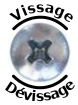
\includegraphics[width=\formCoefficient*\columnwidth]{pics/sens-vissage.pdf}
\end{minipage}

%TODO http://tex.stackexchange.com/questions/30081/how-can-i-sum-two-values-and-store-the-result-in-other-variable/30083#30083

\textbf{Différents tournevis~:} Il existe différentes formes et tailles de tournevis, utiliser la plus adaptée permet de préserver l'empreinte de la vis ainsi que de protéger l'extrémité de l'outil.

\begin{center}
%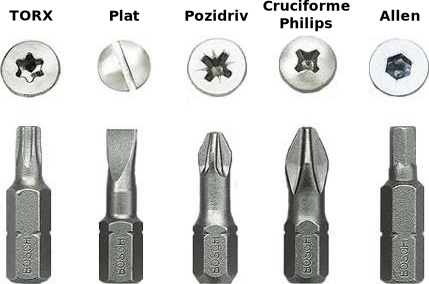
\includegraphics[width=\tailleImageTournevis]{pics/types-tournevis.jpg}
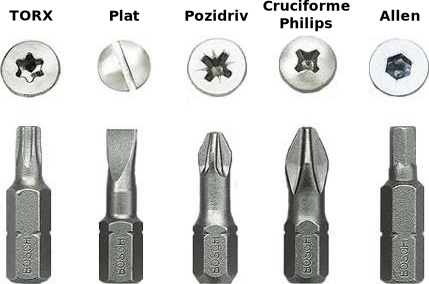
\includegraphics[width=\tailleImageTournevis]{pics/types-tournevis.pdf}
%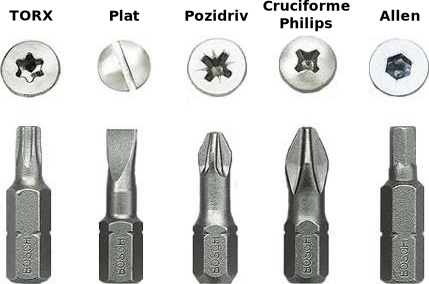
\includegraphics[width=\tailleImageTournevis]{pics/types-tournevis.png}
\end{center}

\textbf{Les clefs~:}  Elles servent à serrer et desserrer les vis, les boulons, et les écrous. Adaptez la dimension de la mâchoire de votre clef à la dimension de l'objet que vous devez, en vous aidant de la molette de la clef, il ne reste plus qu'à visser. \todo{Parler aussi des clefs à pipes, clefs plate, ...}

\textbf{Types de vis~:} pour différents matériaux à utiliser avec le bon tournevis.

\begin{center}
\includegraphics[width=\tailleImageTournevis]{pics/types-vis.jpg}
\end{center}


\section{Perçeuse et Viseuse}
Lorem ipsum dolor sit amet, consectetur adipiscing elit. Nulla enim quam, porttitor sed massa vel, aliquet sagittis tortor. Suspendisse est eros, faucibus non vehicula eget, rutrum at purus. Aliquam auctor vehicula purus, consequat luctus lectus iaculis ultrices. Aliquam tempor dictum ullamcorper. Ut a facilisis lorem, vel tempus eros. Sed elit odio, feugiat vel molestie id, congue in nisl. Aliquam id erat non mi dapibus vulputate. Suspendisse potenti. Aenean tincidunt porta dapibus. Donec euismod eleifend urna, nec pharetra ex iaculis quis.

Lorem ipsum dolor sit amet, consectetur adipiscing elit. Sed malesuada laoreet libero, vitae eleifend metus ultricies eget. Quisque ultrices turpis et orci congue dapibus volutpat sed massa. In lacinia nulla vitae augue imperdiet porttitor. Fusce porta mauris sit amet purus elementum, eget rhoncus lacus tincidunt. Fusce a tempor elit, nec varius erat. Fusce nec vestibulum erat. Vestibulum in lobortis mauris. Phasellus eu volutpat magna, et semper odio. Interdum et malesuada fames ac ante ipsum primis in faucibus. Praesent enim sem, hendrerit eget dictum vel, vehicula vel felis. Suspendisse ultricies eget ex et ullamcorper. Phasellus vitae tellus tincidunt augue gravida ultricies. Mauris gravida lectus vel velit varius, vitae vulputate justo aliquam.


\section*{Fer à souder}
Un fer à souder est un outil permettant de souder deux composants entre eux en faisant fondre un métal d’apport (fil de plomb et d’étain). Il est constitué d’un manche en plastique, d’une partie métallique chauffante et d’une panne.

\textbf{Un fer à souder est par définition très chaud~:} Éloignez tout matériau inflammable du plan de travail (attention aux vêtements et aux cheveux). Il faut toujours le manipuler par le manche en plastique, et ne jamais toucher la partie métallique. Le fer doit toujours être reposé sur un support stable prévu à cet effet entre chaque utilisation. Ne pas utiliser de gants jetables en latex pour se protéger les mains, car ceux-ci peuvent fondre sous la chaleur, et devenir très dangereux.

\textbf{Le métal d’apport est constitué de produits toxiques (plomb, étain)~:} Il est donc important de ne pas respirer les vapeurs issues de la soudure et de travailler dans un local aéré. Il faut toujours se laver les mains une fois la soudure finie, ne jamais mettre le fil de soudure à la bouche, et ne pas souder à proximité de nourriture.

\todo{Insérer image refaite d'n fer à souder}

\begin{itemize}
\item Toujours nettoyer son plan de travail avant et après la soudure.
\item L’embout du fer à souder doit être nettoyé régulièrement à l’aide de l’éponge prévue à cet effet (et seulement à cet effet).
\item Ne jamais souder sur un appareil sous tension. Vérifiez toujours que l’appareil est bien débranché et qu’aucune pile n’est présente.
\item Enfin, après utilisation, veilliez à ce que le fer soit bien éteint et correctement rangé.
\end{itemize}


\section*{Colles et Pistolet à colle}
\subsection*{Pistolet à colle}
Le pistolet à colle est un outil qui permet de faire des collage précis avec des colles puissantes. Il fait fondre un bâtonnet de colle à haute température qui est appliqué grâce à une buse. Le pistolet à colle doit être préchauffé (quelques minutes) avant utilisation.

Ne pas toucher les éléments chauffants, la buse, colle et le bâtonnet sont amenés à haute température et peuvent causer des brûlures. Reposez le pistolet sur son support, pour éviter de coller ce qui ne devrais pas l'être (outils, matériaux, soi-même). Ne respirer pas les vapeur de colle ! La plupart de colles émettent des vapeur toxique lorsqu'elle sont fondues. N'hésitez pas à mettre un masque pour vous protéger.

Il existe plusieurs type de bâtonnets de colle pour cet outil. Il y a certaines colle qui sont adaptées aux différents matériaux, des colles isolante, à prise rapide, etc. Renseignez vous sur la colle la plus adaptée à vos besoins et lisez attentivement les précautions pour chaque colles.

Évitez tout contact avec la colle ! Certaines colles fondue ne peuvent pas être enlevée sans opérations chirurgicale et peuvent laisser des marque à vie. Protégez vos mains avec des gants qui ne sont pas en plastique/caoutchouc car au contact de la colle il pourrais fondre et vous blesser.

\subsection*{Colles}
\todo{TODO}


\section*{Scie sauteuse} % [et disqueuse]}
Une scie sauteuse est un outil de découpe qui utilise une lame entraînée de bas en haut pour couper (d'où le nom de "sauteuse"). Il faut donc faire bien attention à ce mouvement de va et vient de cette lame pour ne pas se blesser ou abîmer le matériel proche de la zone de coupe.

Choisir une lame adaptée au matériau à couper~:
\begin{itemize}
\item petites dents pour les métaux, \textbf{Utiliser de l'huile et lames de type HSS.}
\item dents larges et alternées pour les découpes grossières dans du bois,
\item dents petites et alternées pour les découpes précises dans du bois,
\item \textbf{souvent marqué sur la lame}.
\end{itemize}

Choisir sa vitesse~:
\begin{itemize}
\item vitesse réduite pour les plastiques et métaux,
\item vitesse élevée pour le bois.
\end{itemize}

Attention à bien garder une \textbf{orientation constante} de la lame ; l'appareil peut tourner mais ne pas le pencher dans un sens puis l'autre.

Après une coupe les bords peuvent être coupants (surtout pour les métaux), pensez donc à «ébarber» à la lime ou à l'abrasif (ex: papier de verre).


\section{Contact}

\begin{tabular}{ll}
Mail~: & \url{astups@gmail.com} \\
Forum~: & \url{http://astups.forumactif.com} \\
GitHub~: & \url{https://github.com/astups} \\
\end{tabular}

\end{document}
